\documentclass{report}
\usepackage[utf8]{inputenc}
\usepackage[UTF8]{ctex}
\usepackage{xcolor}
\usepackage{tikz}
\usepackage{clrscode}
\usepackage{booktabs}
\usepackage{mdframed}
\usepackage{amsmath}  %使用宏包,这里使用的是调用公式宏包,可以调用多个宏包
\usepackage{wrapfig}
\usepackage{hyperref}
\usepackage{graphicx}
% \usepackage{booktabs}
% \usepackage{subfigure}
\usepackage{setspace}
\date{}
\usepackage{eso-pic}
\newcommand\BackgroundPic{%
\put(0,0){%
\parbox[b][\paperheight]{\paperwidth}{%
\vfill
\centering

\includegraphics[width=\paperwidth,height=\paperheight,%
keepaspectratio]{cover.jpg}%
\vfill
}}}
\RequirePackage{url}
%Options: Sonny, Lenny, Glenn, Conny, Rejne, Bjarne, Bjornstrup
\usepackage[Rejne]{fncychap}
\usepackage{float}
\newtheorem{theorem}{定理}[section]
\newtheorem{tips}{提示}[section]
\newtheorem{lemma}[theorem]{引理}
\newtheorem{proposition}[theorem]{命题}
\newtheorem{proof}{证明}[section]
\newtheorem{definition}{定义}  
\newtheorem{example}{例子}[section]
\newtheorem{exercise}{习题}[section]
\newtheorem{problem}[exercise]{问题}
\definecolor{mygray}{gray}{0.95}
\definecolor{lightdark}{gray}{0.55}
\definecolor{dark}{gray}{0.3}
\definecolor{skillbg}{gray}{0.7}
\usepackage{algorithm}  
\usepackage{algorithmicx}  
\usepackage{algpseudocode}  
\floatname{algorithm}{算法}  
\renewcommand{\algorithmicrequire}{\textbf{输入:}}  
\renewcommand{\algorithmicensure}{\textbf{输出:}}  
\hypersetup{
	colorlinks=true,
	linkcolor=blue
}
\usepackage{geometry}
\geometry{left=3.18cm,right=3.18cm,top=2.54cm,bottom=2.54cm}
\usepackage{graphicx}
\pagestyle{plain}	
% \usepackage{booktabs}
% \usepackage{subfigure}
\usepackage{setspace}
\date{}
\usepackage{eso-pic}
\newcommand\BackgroundPic{%
\put(0,0){%
\parbox[b][\paperheight]{\paperwidth}{%
\vfill
\centering

\includegraphics[width=\paperwidth,height=\paperheight,%
keepaspectratio]{cover.jpg}%
\vfill
}}}
\begin{document}
\AddToShipoutPicture*{\BackgroundPic}
	\begin{center}
		\quad \\
		\quad \\
		\heiti \fontsize{45}{17} \color{white}{近世代数总结
		\vskip 3.5cm
		\heiti \zihao{2} 近世代数初步	}
	\end{center}
	\vskip 3.5cm

	\begin{quotation}
		\songti \fontsize{15}{15}
		\doublespacing
		\par\setlength\parindent{12em}
		\quad 

		\color{white}{学\hspace{0.61cm} 院:\underline{数学学院\quad}

		专\hspace{0.61cm} 业:\underline{统计学}

		学生姓名:\underline{\qquad OscarLi\qquad }}

		\vskip 2cm
		\centering
		2019年12月14日
	\end{quotation}
\begin{tabular*}{\textwidth}{ccc}
	\includegraphics{figure/by-nc.eps}
	& \begin{minipage}[b]{0.6\textwidth}
		\small\sffamily
		\color{red}{本作品采用知识共享 署名-非商业性使用 4.0 国际 许可协议进行许可.访问} \url{http://creativecommons.org/licenses/by-nc/4.0/  }查看该许可协议.
	\end{minipage}
\end{tabular*}  
 \tableofcontents
\chapter{Group}
\subsection{群的定义}
 \begin{definition}\textbf{群的定义}
 
\noindent$(i):\forall a \in G,\exists a^{-1},a \cdot a^{-1}=e$ (\textcolor{magenta}{可逆性})\\
$(ii):$封闭性 
 \end{definition}
群的判定定理:\\
$\forall a,b\in G,\exists x,y,ax=b \quad and \quad ya=b$(\textcolor{magenta}{证明这个的话,我们只需取a,a的话,我们就可以先把单位元确定了,然后利用性质自然逆元就得到了})\\
性质:
\\在群里消去律是成立的
\begin{proof}
    ac=bc$\rightarrow acc^{-1}=bcc^{-1} \rightarrow a=b $
\end{proof}
 \begin{definition}(半群的定义:)
\\半群只要求满足结合律(幺半群有单位元)
 \end{definition}
\subsubsection{交换群}
 \begin{definition}\textbf{交换群}
 $\forall a,b \in G,ab=ba$
  \end{definition}
\subsubsection{子群}
 \begin{definition}\textbf{子群}
\noindent 设G是一个群,H是G的一个非空子集,如果H关于G的运算也构成群,则称H为G的一个子群 ,记为$H<G$
 \end{definition}
子群的判定定理:$H\subset G,\forall a,b \in H,if ab^{-1} \in H,\rightarrow$H为G的子群
\subsection{陪集\quad 正规子群}
\begin{definition}\textbf{陪集:}
\noindent $H<G$ 
$a H=\{a h | \forall h \in H\}$
\end{definition}

\begin{definition}$\star$ \href{https://ncatlab.org/nlab/show/normal%20subgroup}{\textbf{正规子群:}}
\noindent $\forall a \in G \quad a H=H a$ 
则我们记作$H \triangleleft G$
\end{definition}
\begin{mdframed}[backgroundcolor=blue!7] 
\noindent 关于正规子群的等价性命题:
	$$\forall a \in G,aHa^{-1}=H$$
	$$\forall a \in G,aHa^{-1}\subseteq H$$
	$$\forall a \in G,h \in H,aha^{-1}\in H$$
\end{mdframed}
\subsubsection{商群}
\noindent 商群的概念结合了陪集与正规子群
\begin{definition}\textbf{商群}
$如果 H \triangleleft G \quad ,$
$G/H$称为商群
\end{definition}
\subsection{群同态与同构}
\begin{definition}\textbf{群同态}
\noindent $f:(G,\cdot)\rightarrow(H,\triangle)$
\\$f(g_{1}\cdot g_{2})=f(g_{1})\triangle f(g_{2}))$
\end{definition}
\begin{definition}
\noindent f为单射 $\rightarrow $单同态
\\ f为满射 $\rightarrow $满同态
\\ f为双射 $\rightarrow$同构
\end{definition}
\noindent 单位元具有唯一性: \\
\begin{proof}
	$f\left(e_{1}\right)=f\left(e_{1}^{2}\right)=f\left(e_{1}\right) \Delta f\left(e_{1}\right)=\left[f\left(e_{1}\right)\right]^{2}$
	
	\end{proof}
\subsection{群同态基本定理}
\subsubsection{群同态基本定理}
\begin{theorem}
\noindent f :G$\rightarrow H$
\\(G,$\cdot$)$\rightarrow(H,\triangle)$
\\$\frac{G}{Kerf}\cong Imf$
\\\textcolor{magenta}{$\left\{Kerf=g|f(g)=e_{H}\right\} \quad and \quad Imf=\left\{f(g)|g \in G \right\}$}
\end{theorem}
\begin{proof}
	从单射开始说起,
	令gKerf=$\bar{g}$
		\end{proof}
		\subsubsection{群同构第二定理}
		\begin{theorem}
		$N \triangleleft G,H < G
		 \rightarrow  $
		
			$\left. H \middle/ N \cap H \right.\cong \left. NH \middle/ N 
	\right.$
		\end{theorem}
		
		\subsubsection{群同构第三定理}
		\begin{theorem}
			$N \triangleleft G,H \triangleleft G,$
			$G \big/ N \bigg/ H \big/  N  \cong \left. G \middle/ H
	\right.$
		\end{theorem}
\subsection{循环群分类定理}
\begin{theorem}
$$ \left\{
\begin{aligned}
(a_{m}) \cong Z_{m} 
\\
(a)\cong Z
\end{aligned}
\right.
$$
\end{theorem}
\subsection{Cayley定理}
\begin{definition}
任何一个群都同构于一个对称群的子群
\end{definition}

\subsection{Lagrange定理}
\begin{theorem}
\noindent $H<G$
\\G为有限群的情况,H的阶整除G的阶 \\
\end{theorem}
\begin{problem}
素数阶的群一定是循环群?
\end{problem}

\subsection{群的作用}
\begin{definition} \href{https://ncatlab.org/nlab/show/action}{群的作用:}\\ $\varphi:G \times S \rightarrow S$
\\(g,s)$\rightarrow g(s)$
\end{definition}

\begin{framed}
	\noindent 共轭作用$ f $:G为群,$\forall a,b\in G,f(b)=a^{-1}ba$
\end{framed}
\noindent\textcolor{magenta}{群的作用一定是双射}
\subsubsection{轨道与稳定子}
\noindent $Orb(s)=\left\{g(s)|g \in G\right\}$
\\
$Stab(s)=\left\{g\in G|g(s)=s\right\}$
\begin{theorem}
设G在S上有一个群作用,则(1)S=ord(S)
\end{theorem}
\subsubsection{群的类方程}
\begin{framed}
	\noindent 环的中心:$C(G)= \{ a \in G|\forall g \in G,ag=ga \}$
\end{framed}
\subsection{Sylow定理}
\begin{framed}
\noindent 杨老师说这个可以理解成seelow定理(这个定理可以一览众山小)
\end{framed}
\noindent P群:G为有限群,|G|为某个素数P的方幂$P^{k},(k \geq 1)$,则称G为一个p群 \\
\noindent \href{https://ncatlab.org/nlab/show/Sylow%20p-subgroup}{Sylow p-群:} 
Sylow p-群其实是一个很有意思的概念,这个概念如果只是盯着群本身的话,很难理解它的重要性,我们要重新看看之前的概念,像子群,就会发现这概念的有意思的地方
\subsubsection{Sylow第一定理}
\begin{theorem}
假设G为有限群,p为素数,|G|=$p^{n}m,0<k \leq n$,则G有阶数为$p^{k}$的子群
\end{theorem}
\begin{deduction}
对于有限群G,|G|的任一素因子p,G有Sylow p群
\end{deduction}
\subsubsection{Sylow第二定理}
\begin{theorem}\textbf{Sylow第二定理}
设H为有限群G的p-子群(不一定是Sylow p-子群)且P为G的Sylow P-群
\\则 $\exists x \in G,s.t:H $
\end{theorem}
\begin{deduction}
Sylow p-群彼此共轭
\end{deduction}
\subsubsection{Sylow第三定理}
\begin{theorem}
有限群G的sylow p子群的个数$n_{p}$是G的因子且满足同余式:

\end{theorem}
\begin{exercise}
计算阶为200群的Sylow-p群的个数:
\end{exercise}
\begin{definition} \textbf{单群}
单群:除平凡群以外,没有正规子群
\end{definition}
\section{Ring }

\subsection{环的定义}
\begin{definition} \textbf{环的定义}
\noindent $(i)(\mathbb{R},+)$构成一个交换群 \\
$(ii)(R,\cdot)$满足结合律 \\
$(iii)(R,+,\cdot)$满足分配律\\
\end{definition}
\begin{proposition}
若环K中没有零因子,则消去律成立
\end{proposition}
\begin{definition}\textbf{交换环}
若$ab=ba,\forall a,b \in R$交换环
\end{definition}
\subsubsection{子环}
\begin{definition}\textbf{子环}
\noindent$(R,+,\cdot)$是一个环,S为R的一个非空子集,S关于R的运算成环,则称S为R的子环
\end{definition}
\noindent$(R,+,\cdot)$是一个环,S为R的一个非空子集,则S为R的子环的充分必要条件:
\\(i)(S,+)为(R,+)的加法子群
\\(ii)$\forall a,b \in S\rightarrow ab \in S $

\subsection{域,除环,体}
\begin{definition}\textbf{零因子:}
$a \neq 0,\exists b \neq 0,使得ab =0$
\end{definition}
这里我们注意,零因子的概念重要性从反面而言,是很显然的,在日常生活中的常用的代数结构,$\mathbb{R}$,除开零元来看的话,都是没有零因子这种代数结构的
\begin{mdframed}
 这里注意零因子与零元不是一个概念
\end{mdframed}
\begin{definition}\textbf{无零因子环}
无零因子环:我们把没有零因子,有单位元e的环称为无零因子环
\end{definition}
\begin{definition}\textbf{整环}
一个没有零因子,有单位元e的交换环R称作整环
\end{definition}
\begin{example}
高斯整环:$Z[i]$
\end{example}
$(R,+,\cdot)$满足结合律,则称为域

\begin{example}
\noindent 四元数体(Hamilton quaternion field)=$\left\{a+bi+cj+dk|a,b,c,d\in R\right\}$
\end{example}
\begin{definition}\textbf{除环}
R有单位元$e \neq 0$的环,在环中非零元都可逆
\end{definition}
\begin{definition}\textbf{域}
F为一个有单位元的交换环,如果每个非零元都可逆,则称为域
\end{definition}
\begin{problem}
$Q \sqrt[3]{2}$
\end{problem}
\subsection{环同态}
\begin{definition}\textbf{环同态}
设$R_{1},R_{2}$为两个环,\\
$$f:R_{1} \rightarrow R_{2}$$
\end{definition}
若f满足:
\\(i)$f(r_{1}+r_{2})=f(r_{1})+f(r_{2})$
\\(ii)$f(r_{1}r_{2})=f(r_{1})f(r_{2})$
\subsection{理想}
\begin{definition}\textbf{理想}
\noindent R为环,I为R的非空子集,如果I满足:
\\$(i)\forall r_{1},r_{2}\in I,r_{1}-r_{2}\in I$\\
$(\forall r \in R,\forall i \in I),ri \in I$称为左理想$ir \in T$称为右理想
\end{definition}
\subsubsection{商环}
\begin{definition}\textbf{商环}
环R,理想I,在(R,+)的商集$R \bigg/ I = \{r+I|r \in R \}$上
\end{definition}
\subsubsection{主理想}
\begin{definition}
\href{https://ncatlab.org/nlab/show/ideal}{主理想}
R为环, $\forall a \in R,$,则(a)=由a生成的理想,称为主理想

\end{definition}
这个概念比较麻烦,我们康康一个例子,
\begin{example}
设R为有单位元的交换环,则主理想:$(a)={ra|r \in R}$
\end{example}
\begin{proof}
    (i)首先证明(a)为R的一个子环,
    $ \forall \alpha,\beta \in (a), \rightarrow \alpha =r_{\alpha}a,\beta= r_{\beta}a$
    \\我们利用子环的判定定理\\
    易知$\alpha - \beta =(r_{\alpha}-r_{\beta})a \in (a)$
    \\$\alpha \beta =r_{\alpha}r_{\beta}aa \in (a)$($r_{\alpha}r_{\beta} \sim r$)
    \\(ii)我们还要考虑一些事情:(a)本身为理想,
   \\  $\forall \bar{r} \in R, \bar{r}(a)= \lbrace \bar{r}ra \rbrace$
   \\ $\bar{r}(a) \subset (a) $
\end{proof}

\subsubsection{极大理想与素理想}
\begin{definition} \textbf{极大理想}
R为交换环,M为R的真理想,对R的任一包含M的理想N $\rightarrow N=M \quad Or \quad N=R$
\end{definition}
        \begin{definition}\href{https://ncatlab.org/nlab/show/prime%20ideal}{\textbf{素理想}}
\noindent R为交换环,P为R的真理想,如果$\forall a,b\in R$,由 $ab\in P \rightarrow a \in P \quad Or \quad b \in P$
\end{definition}
\begin{proposition}
R为一个有单位元的交换环,则R的每个极大理想都是素理想

\end{proposition}
\subsection{主理想环}
\begin{definition}
环的每一个理想都是主理想
\end{definition}
\begin{example}
除环,域都是主理想
\end{example}
\begin{example}
$$(\mathbb{Z},+,\times)$$
主理想整环
\end{example}
\subsection{多项式整环}
\begin{definition}\textbf{多项式整环}
(\textbf{R}(x),+,$\times$)
\\ $P_{1}(x)=a_{n}x^{n}+a_{n-1}x^{n-1}+\dots+a_{1}x+a_{0}$

\end{definition}
\subsection{域的扩张}
\begin{definition}
$K \subset \mathbb{F}$,为两个域,称$\mathbb{F}$为K的扩域
\end{definition}
\subsection{代数元,超越元}
\begin{definition}\textbf{代数元}
设$\mathbb{F}$是一个域,称$\alpha$为代数数,若存在一个多项式f(x)$\in \mathbb{F}[x] ,s.t. f(\alpha)=0$
\end{definition}
\subsection{极小多项式}
\begin{definition}
$\mathbb{F}$为域,

\end{definition}
\begin{proposition}
极小多项式不可约
\end{proposition}
\section{习题}
\subsection{群}
\begin{problem}
证明正规子群的等价性命题:
	$$\forall a \in G,aHa^{-1}=H$$
	$$\forall a \in G,aHa^{-1}\subseteq H$$
	$$\forall a \in G,h \in H,aha^{-1}\in H$$
\end{problem}
\begin{Hint}
$$\forall a \in G,h \in H,aha^{-1}\in H$$
\\ 我们从这里证明正规子群,
\textcolor{lightdark}{$ah=aha^{-1}a=(aha^{-1})a \subset Ha
\\ \forall a \in G ,a^{-1}h(a^{-1})^{-1} \in H ,\rightarrow ha \in aH,Ha \subset aH
$}
\end{Hint}
\begin{exercise}
f:$G \rightarrow H$群同态
\\ 则$ Kerf \triangleleft G$
\end{exercise}
\begin{Hint}
\textcolor{lightdark}{$\forall gkg^{-1} \in g Kerf g^{-1}
\\ f(gkg^{-1})=f(g)f(k)f(g^{-1})
\\ =f(g)e_{H}[f(g)]^{-1}=e_{H}
\\ gkg^{-1} \in Kerf(gKerfg^{-1}\subset Kerf)$}
\end{Hint}
\begin{problem}
证明群同态基本定理f :G$\rightarrow H$
\\(G,$\cdot$)$\rightarrow(H,\triangle)$
\\$\frac{G}{Kerf}\cong Imf$

\end{problem}
\begin{proof}
\textcolor{lightdark}{Kerf显然是正规子群,}
\end{proof}
\begin{exercise}
设$C(G)= \{ a \in G|\forall g \in G,ag=ga \} $,是群G的中心,证明:如果G/C(G)是循环群,则G是Abel群
\end{exercise}
\begin{exercise}
简要证明Sylow定理(1,2,3)
\end{exercise}
\begin{exercise}
设 G 的阶为 168, G 中有多少个阶为 7 元素
\end{exercise}
\subsection{环}
\begin{exercise}
在$\mathbb{Z}_{2}[x]$中多项式$x^3+x^2+1$是不可约的,并利用这一结论构造一个有8个元的有限域
\end{exercise}
\begin{proof}
\textcolor{lightdark}{在数域$\mathbb{Z}_{2}[x]$只有$\bar{1},\bar{0}$,容易得出多项式$X^3+X^2+1$是不可约的(其值不为0),利用$f(x)$不可约$\rightarrow$ $(f(x))$为极大理想
\\  $\mathbb{Z}_{2}[x] \bigg/ (x^3+x^2+1)$是域
={$\bar{a}+\bar{b}x+\bar{c}x^2$}(2*2*2)
}
\end{proof}
\begin{exercise}
求环$\mathbb{Z}_{28}$的所有素理想和极⼤理想
\end{exercise}
$$
\begin{cases}
(a_{m}) \cong Z_{m} 
\\
(a)\cong Z
\end{cases} $$
\end{document}






